%% LyX 2.3.7 created this file.  For more info, see http://www.lyx.org/.
%% Do not edit unless you really know what you are doing.
\documentclass[english]{article}
\usepackage[T1]{fontenc}
\usepackage[latin9]{inputenc}
\usepackage{geometry}
\geometry{verbose,tmargin=1in,bmargin=1in,lmargin=1in,rmargin=1in}
\setlength{\parindent}{0bp}
\usepackage{mathtools}
\usepackage{amsmath}
\usepackage{amssymb}
\usepackage{graphicx}
\usepackage{setspace}
\doublespacing
\usepackage{babel}
\begin{document}

\section*{Numerical Solution}

Let us now examine a numerical solution. For this section we will
use a different friction model, decribed later.

We start with our PDE:

\[
A_{c}EU_{xx}+f_{x}(x,t)=\rho U_{tt}+\mu_{k}U_{t}+F_{dry}(U_{t})
\]

We will use the Explicit Finite Difference Method to numerically solve
our PDE. To do so we will discretize $U$ as follows:

\[
U_{j}^{n}\coloneqq U\left(j\Delta x,n\Delta t\right)
\]

where $j=1,2,...,J$, $n=1,2,...,N$, and $\Delta x$ and $\Delta t$
are small changes in $x$ and $t$, respectively. We will use the
following finite difference appriximations:

\[
U_{t}\left(j\Delta x,(n+1)\Delta t\right)\thickapprox\frac{U_{j}^{n+1}-U_{j}^{n}}{\Delta t}
\]
 

\[
U_{tt}(j\Delta x,(n+1)\Delta t)\thickapprox\frac{U_{j}^{n+1}-2U_{j}^{n}+U_{j}^{n-1}}{(\Delta t)^{2}}
\]
 

\[
U_{xx}(j\Delta x,(n+1)\Delta t)\thickapprox\frac{U_{j+1}^{n}-2U_{j}^{n}+U_{j-1}^{n}}{(\Delta x)^{2}}
\]
 

We have a problem of defining $U_{xx}$ when $j=1$ or $J$, so we
will set $U_{xx}\left(1,n+1\right)=U_{xx}\left(2,n+1\right)$ and
$U_{xx}\left(J,n+1\right)=U_{xx}\left(J-1,n+1\right)$. Since $F_{dry}$
is nonlinear, we will approximate $F_{dry}(U_{t})\thickapprox F_{dry}\left(\frac{U_{j}^{n}-U_{j}^{n-1}}{\Delta t}\right)$.
This may not be ideal and both could be a source of error. However,
if $\Delta x$ and $\Delta t$ are small enough, this error should
be small. Substituting these into our PDE we get the following. 

\[
A_{c}E\frac{U_{j+1}^{n}-2U_{j}^{n}+U_{j-1}^{n}}{\left(\Delta x\right){}^{2}}+f_{x}(x,t)=\rho\frac{U_{j}^{n+1}-2U_{j}^{n}+U_{j}^{n-1}}{\left(\Delta t\right){}^{2}}+\mu_{k}\frac{U_{j}^{n+1}-U_{j}^{n}}{\Delta t}+F_{dry}\left(\frac{U_{j}^{n}-U_{j}^{n-1}}{\Delta t}\right)
\]

Solving for $U_{j}^{n+1}$ we get:

\[
U_{j}^{n+1}=\frac{A_{c}E\frac{U_{j+1}^{n}-2U_{j}^{n}+U_{j-1}^{n}}{\left(\Delta x\right){}^{2}}+f_{x}(x,t)+\rho\frac{2U_{j}^{n}-U_{j}^{n-1}}{\left(\Delta t\right){}^{2}}+\mu_{k}\frac{U_{j}^{n}}{\Delta t}-F_{dry}\left(\frac{U_{j}^{n}-U_{j}^{n-1}}{\Delta t}\right)}{\frac{\rho}{\left(\Delta t\right){}^{2}}+\frac{\mu_{k}}{\Delta t}}
\]

We can use this to solve $U(x,\Delta t\,(n+1))$ given $U(x,\Delta t\,n)$
and $U(x,\Delta t\,(n-1))$ .

We will define the initial conditions $U_{j}^{0}\coloneqq U_{j}^{1}\coloneqq0$.
We will set $\Delta x=\frac{1}{20}$, $\Delta t=\frac{1}{800}$, $J=21$,
$N=81$, $A_{c}=0.1964$, $E=5\times10^{-5}$, $\rho=1100$, and $\mu_{k}=1000$.
$A_{c}$is the cross sectional area, $E$ is Young's Modulus of the
body, $\rho$ is the density, and $\mu_{k}$ is the constant for dry
friction. Many of these values we got from the paper, Excitation of
Faraday-like body waves in vibrated living earthworms, by Ivan S.
Maksymov. We will define:

\[
f_{x}(x,t)=kf_{0}\cos\left(kx-\varpi t\right)
\]

where $k=\frac{3}{2}\pi$, $f_{0}=2000$, and $\varpi=\pi$. We will
also define a piecewise linear model for dry friction, similar to
that used in Friction Compensation Strategy for Feed Servo Systems
Based on Static Friction Model, by Huang, Chen:

\[
F_{dry}\left(U_{t}\right)=\begin{cases}
F_{1}*U_{t}-F_{0} & U_{t}>0\\
0 & U_{t}=0\\
a\,F_{1}*U_{t}-F_{0} & U_{t}<0
\end{cases}
\]

where $F_{1}=10^{4}$, $F_{0}=10^{3}$, $a=5$. 

We can then graph $F_{dry}\left(U_{t}\right)$, and $U(x,t)$. 

\begin{figure}[h]
\hfill{}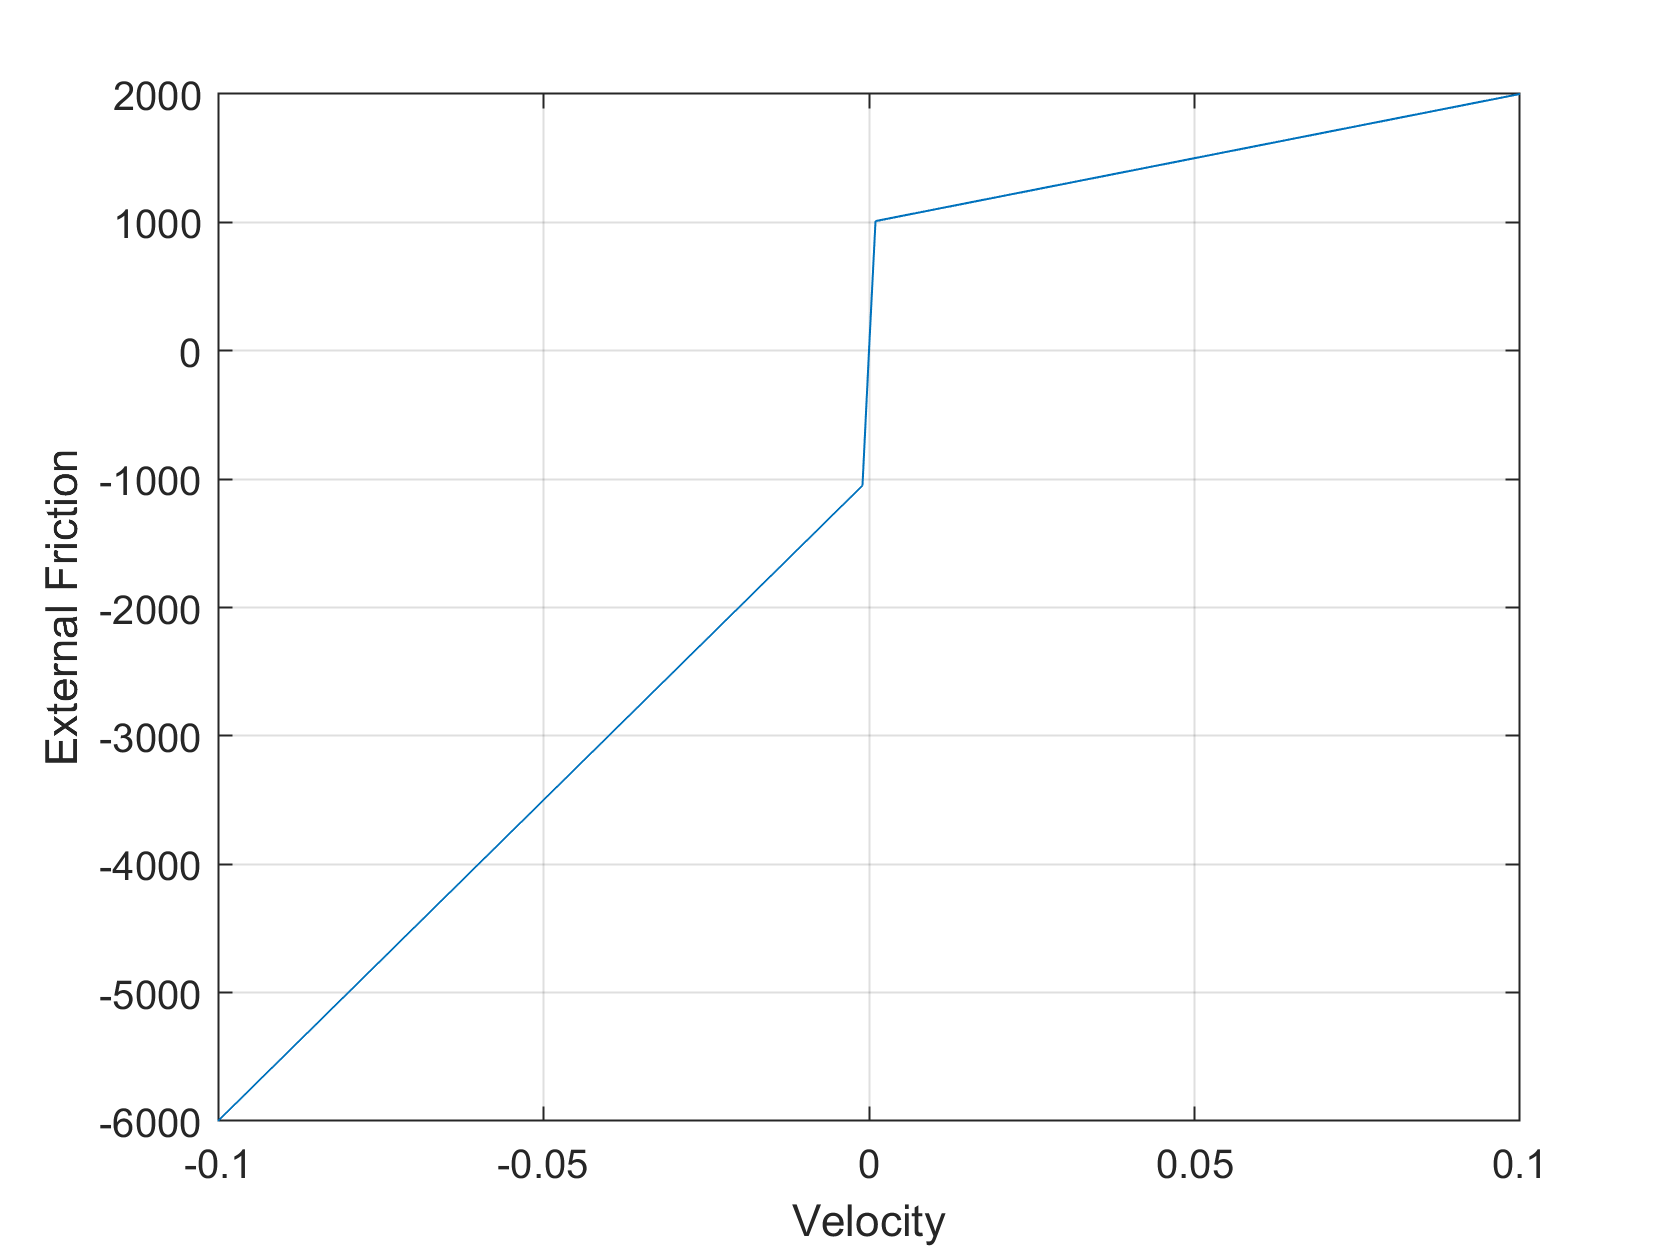
\includegraphics[width=2.8in,height=2.8in,keepaspectratio]{dryFriction}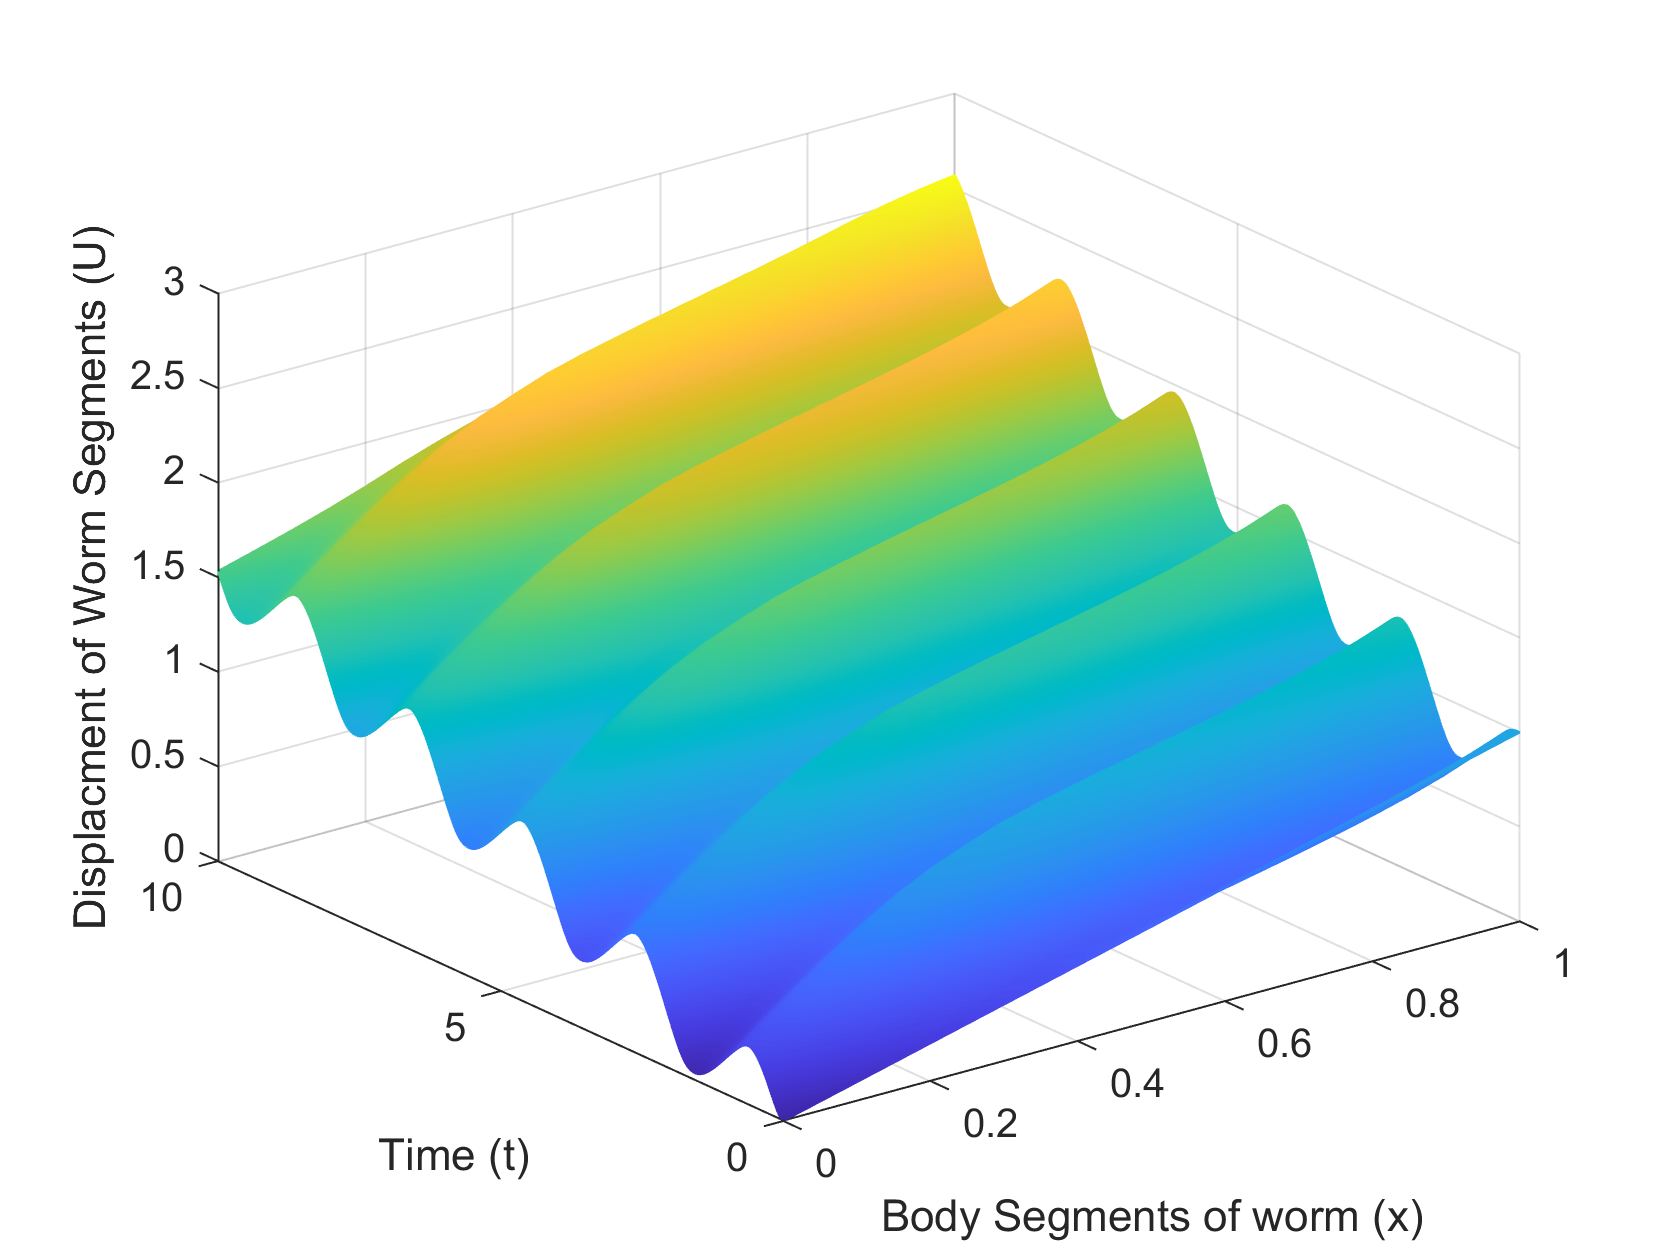
\includegraphics[width=3in,height=3in,keepaspectratio]{3Dgraph_displacment}\hfill{}

\caption{The left graph is $F_{dry}\left(U_{t}\right)$ vs. $U_{t}$. The right
graph is $U\left(x,t\right)$vs. $x$ and $t$.}
\end{figure}

\begin{figure}[h]
\hfill{}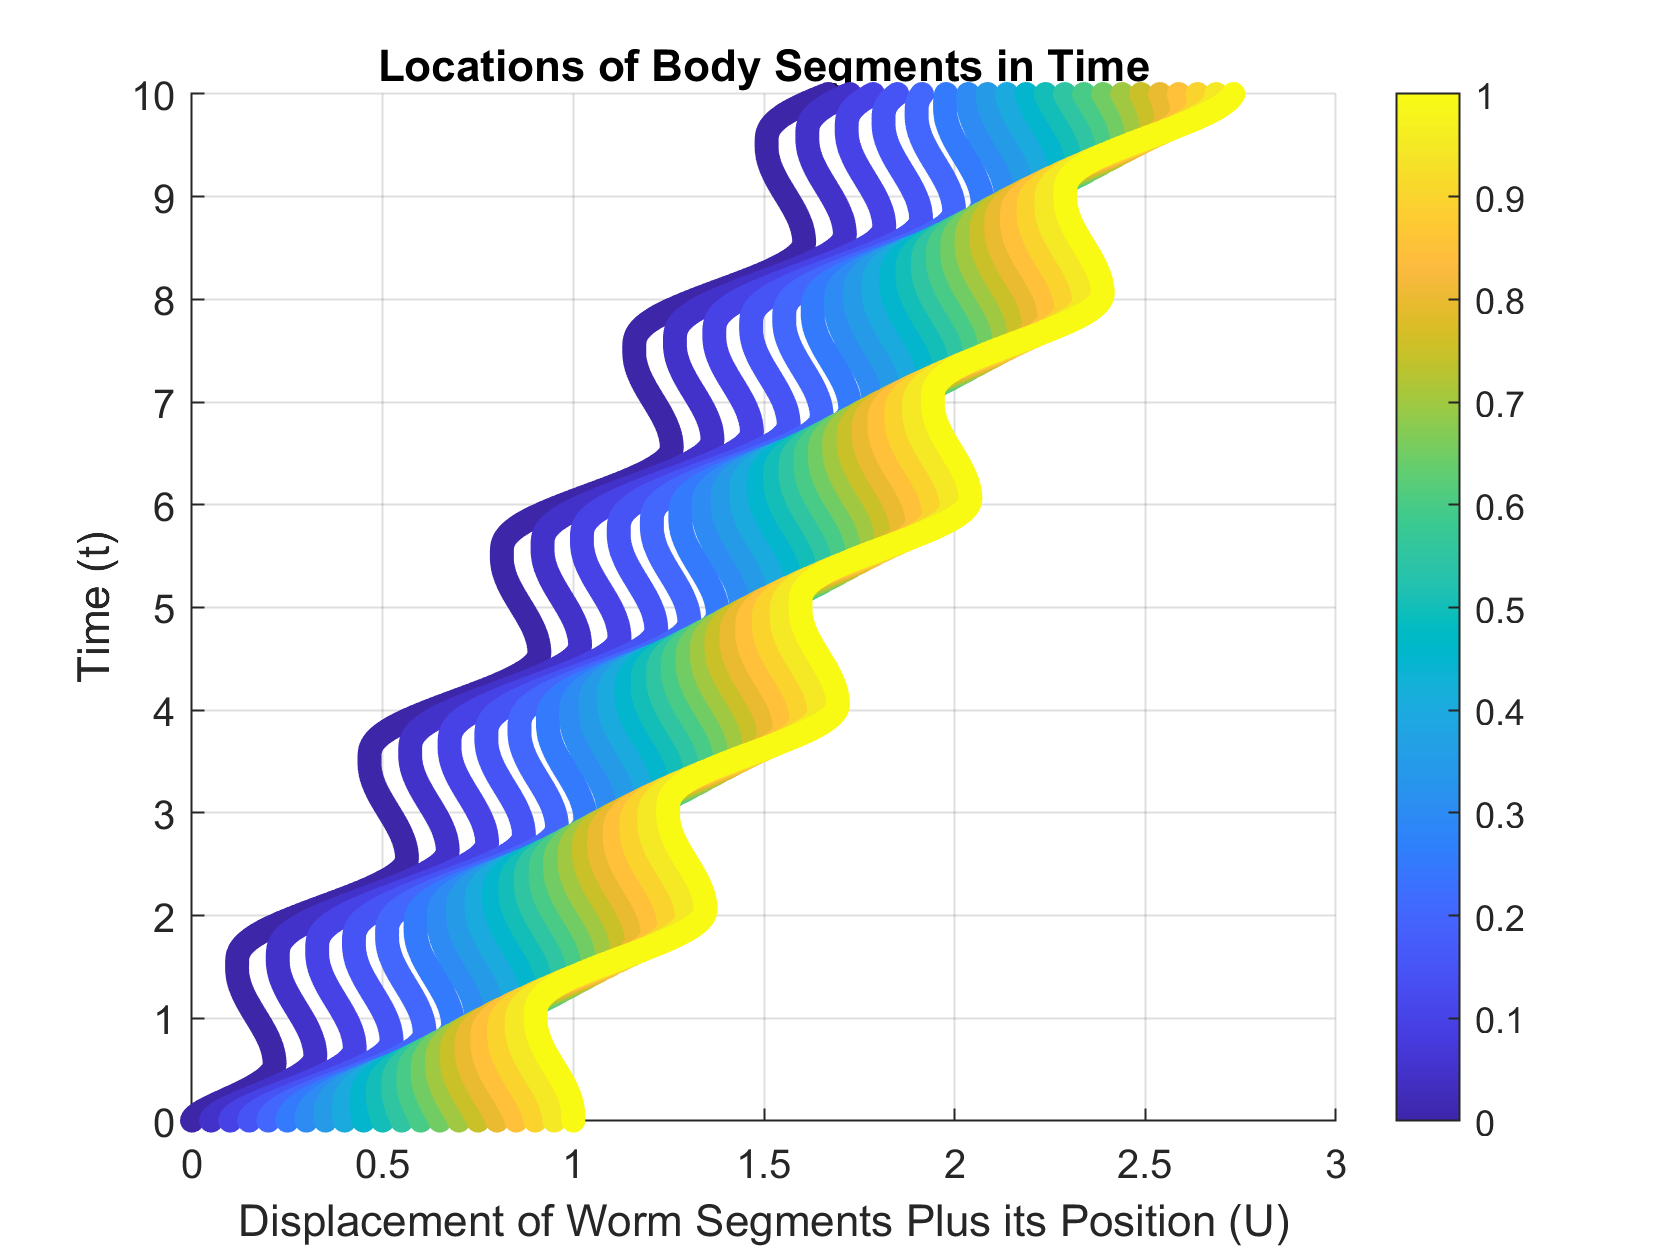
\includegraphics[width=6.5in,height=6.5in,keepaspectratio]{2Dgraph_displacment}\hfill{}

\caption{A graph of $U\left(x,t\right)$vs. $x$ and $t$, where $x$ is represented
by colors.}
\end{figure}

We can see that the $U$ is increasing with time meaning that the
worm is moving forward. We can also see that the movement of the worm
is periodic, as the worm repeatedly contracts and expands.
\end{document}
